% !TeX root = ./00-main.tex
% ============================================================================
% Chapter 4 -- Discussion and Conclusions
% Revised 2026-07-30
% ============================================================================

\chapter{Discussion and Conclusions}
\label{chap:discussion}

\section{Principal findings}
\label{sec:principal-findings}

This thesis asked a deliberately narrow question: during premalignant epithelial progression, does tissue context explain additional progression-aligned regulatory change beyond that predicted from the epithelial receiver itself, and at what spatial scale can that information be recovered? StageBridge addressed this question with a structured universal differential equation that separates an intrinsic progression field from a context-conditioned field and summarizes their endpoint difference as a program-resolved conditional context residual, $R_{\mathrm{cond}}$. Three findings define the answer.

First, the fitted full-versus-self contrast contained a coordinated set of program-level residuals that reproduced under patient-held-out and leave-one-donor-out resampling. On the AAH$\rightarrow$AIS edge, twenty-nine regulatory programs had held-out confidence intervals excluding zero, with concordant signs across all five patient-held-out folds and leave-one-donor-out analyses; twenty-eight programs met the same criterion on the AIS$\rightarrow$invasive edge. The stable programs were not isolated coefficients. They formed interpretable axes involving p53, WNT, TRAIL, AP-1-associated activity, interferon signaling, SMAD4, chromatin coregulation, lineage identity, and metabolic stress. This establishes the resampling stability of the residual structure under the fitted StageBridge decomposition. It does not, by itself, establish that the number of stable programs exceeds a full pipeline retrained under permuted context, an experiment that remains necessary to define an estimand-level context null.

Second, receiver-local context did not provide detectable predictive information beyond matched marginal context. A model supplied with each receiver's local niche had a lower mean endpoint distance than self-only transport and was favored in four of five folds, but the paired difference was not statistically significant ($8.76$ semantic Sinkhorn units, $95\%$ CI $[-2.83,+20.35]$, $P\approx0.10$). More decisively, local context did not separate from a stratum-matched shuffle of the same niche features ($0.08$ units, $95\%$ CI $[-1.10,+1.26]$). Thus, the available evidence does not support the stronger hypothesis that receiver-specific local context improves progression inference. The near-zero local-versus-shuffled contrast was estimated much more precisely than the local-versus-self contrast and therefore provides the clearest falsification result. A variance decomposition offered a plausible explanation: within-specimen variation accounted for approximately $85$--$96\%$ of the observed variation in the selected macrophage, fibroblast, and CAF context features, whereas stage-associated variation was limited. The context information recoverable from these cohorts was therefore predominantly specimen-associated rather than uniquely receiver-local.

Third, the PanIN analysis returned no stable programs. In a four-donor cohort, this outcome is compatible with either a true absence of reproducible residual structure or insufficient power, and those explanations cannot be separated. The analysis nevertheless showed that the pipeline did not over-call patient-robust stability in a cohort unable to support it. It should be interpreted as a boundary of available evidence, not as independent validation or proof of estimator calibration.

The overall result is therefore bounded but informative. StageBridge recovered reproducible program-level residual structure under its fitted decomposition, while the receiver-local niche hypothesis was not supported by the falsification ladder. The central contribution is not an unqualified claim that local context drives progression; it is a program-resolved and patient-held-out framework that distinguishes reproducible modeled context structure from the stronger spatial claim that the available data could not establish. Because the transported state is expressed in named pathway and transcription-factor coordinates, those residuals also provide a direct route from population transport to experimentally testable signaling hypotheses rather than ending at an anonymous vector field.

\section{A reproducible context-associated component of premalignant progression}
\label{sec:biological-interpretation}

Premalignant epithelial progression occurs within tissue ecosystems that change together with the epithelial compartment. Recent spatial studies of lung adenocarcinoma precursors have independently described coordinated remodeling of alveolar progenitor states, inflammatory niches, immune barriers, fibroblasts, and invasive epithelial phenotypes \autocite{Peng2025-xu,Takano2024-gp,Cardoso2026-kp}. StageBridge asks a more restricted question than these atlases: after conditioning the source--target comparison on coarse ecological strata and holding the starting epithelial receiver fixed, what additional regulatory displacement is associated with including context in the fitted field?

\subsection{Preinvasive progression is consistent with de-repression under retained checkpoint stress}

The AAH$\rightarrow$AIS stable set combines increased p53 ($+0.295$), WNT ($+0.293$), TRAIL ($+0.203$), and AP-1-associated FOS ($+0.141$) residuals with decreased SMAD4 ($-0.099$), JAK--STAT ($-0.246$), and IRF9 ($-0.129$) residuals. These coordinates are transcriptional activity footprints rather than direct measurements of mutation, phosphorylation, or protein function \autocite{Schubert2018-ph}. An increased p53 footprint is therefore compatible with oncogenic or genotoxic stress in cells that retain a transcriptional checkpoint response, even if later lesions acquire genomic alterations that compromise the pathway \autocite{Haga2023-xc,Zhao2025-vm}. A similar coexistence of oncogenic and tumor-suppressive programs has been reported in an independent pancreatic model at the benign-to-malignant transition \autocite{Reyes2026-yr}. The cross-disease comparison does not validate the lung coefficients, but it supports interpreting the pattern as a contested transition rather than a simple monotonic activation of malignant drive.

The transcription-factor residuals sharpen that interpretation while remaining mechanistic nominations rather than direct regulatory edges. ETV6, a transcriptional repressor, lost context weight, whereas FOS gained it. Functional studies in Ewing sarcoma show that ETV6 can constrain an oncogenic transcriptional program through chromatin competition, illustrating the broader principle that loss of a repressive factor can release a state-changing program \autocite{Lu2023-yz}. In the present data, the coordinated decrease of several repressor-associated factors alongside increased FOS is consistent with de-repression of an AP-1-associated response; it does not establish that these factors directly regulate FOS in lung precursors. KAT5 also gained context weight ($+0.127$) alongside p53 and RB1. KAT5/TIP60 acetylates p53 after DNA damage and helps determine downstream checkpoint responses \autocite{Tang2006-ns}. Their joint recovery provides biologically coherent support for a checkpoint-stress interpretation, but the activity scores remain model-derived and should not be read as measurements of p53 acetylation.

The same edge shows a coordinated decrease in interferon-associated activity. IRF9 is part of the STAT1--STAT2--IRF9 ISGF3 complex that mediates canonical type-I interferon-induced transcription \autocite{Platanitis2019-av}. Hallmark interferon-$\alpha$ and interferon-$\gamma$ responses were also downregulated by an independent whole-transcriptome enrichment analysis. This direction is consistent with longitudinally annotated bronchial premalignant lesions, in which progressive lesions showed reduced interferon signaling relative to regressive lesions \autocite{Beane2019-mp}. At invasion, STAT5B gained context weight while IRF9 did not, suggesting a change in the dominant JAK--STAT-associated regulator rather than a simple restoration of the same interferon program. STAT5 proteins can transduce cytokine and growth-factor signals into proliferative and metabolic programs \autocite{Li2023-tt}. The phrase ``arm switch'' is therefore useful as a descriptive summary of the fitted residuals, but it should not be interpreted as direct evidence of receptor-level rewiring.

Together, the preinvasive residuals are most defensibly described as a context-associated shift toward epithelial drive and stress adaptation while selected checkpoint programs remain transcriptionally active and interferon tone declines. This interpretation is supported by convergence across pathway scores, regulator scores, gene-set enrichment, and external precursor literature, but remains a model-based description of coordinated programs rather than a validated molecular circuit.

\subsection{Invasion reorganizes lineage and coregulator architecture}

The AIS$\rightarrow$invasive stable set is not simply a larger version of the preinvasive set. HDAC1, CTBP1, and NAB2 lost context weight, while MAML1 and FOXA1 gained it. These changes nominate a shift in coregulator and chromatin-accessibility architecture. MAML1 is a canonical Notch coactivator whose acetylation supports assembly of a transcriptionally active complex \autocite{Jin2017-ph}; it can also act as a p53 coactivator independently of Notch, increasing p53 stability and post-damage activation \autocite{Zhao2007-xt}. FOXA1 is a pioneer factor capable of engaging compacted chromatin \autocite{Lerner2023-bx}. In NKX2-1-positive lung adenocarcinoma, FoxA1 and FoxA2 maintain growth and a plastic pulmonary--gastrointestinal identity state \autocite{Orstad2022-hw}. Increased FOXA1 residual weight at invasion is therefore consistent with lineage plasticity, although StageBridge does not identify the direction of FOXA1 binding or its direct targets in these lesions.

A second invasion-associated group involved ATF5, HSF2, NFKB2, MYC targets, and oxidative phosphorylation. This pattern is consistent with increased biosynthetic and stress-management demands as epithelial identity is reorganized. STAT5B, which gained context weight on the same edge, provides a plausible upstream connection because STAT proteins can coordinate metabolic programs in cancer cells and the tumor microenvironment \autocite{Li2023-tt}. That connection is a hypothesis generated by agreement among fitted programs, not a reconstructed signaling chain.

WNT and TRAIL were the only pathway residuals that remained stable with the same sign on both lung edges. WNT therefore represents the most persistent context-associated program in the fitted model, whereas most other changes were edge-specific. This persistence makes WNT a strong candidate for cross-stage validation, but the present data do not establish therapeutic tractability or stage-independent intervention efficacy. TRAIL also requires careful interpretation. Sustained sublethal death-receptor signaling in apoptosis-resistant cells can produce non-apoptotic NF-$\kappa$B- and JNK-associated outputs \autocite{Azijli2013-tr}; the co-occurring AP-1 and NFKB2 residuals are compatible with that possibility, but the data cannot distinguish non-apoptotic signaling from a pro-apoptotic response.

\subsection{A context residual is not a pathway level}

The VEGF result illustrates why $R_{\mathrm{cond}}$ cannot be read as differential expression or absolute pathway activity. VEGF was the largest-magnitude stable pathway on the invasion edge and was redirected downward ($-0.318$), despite the established relationship between invasion and angiogenesis. The apparent contradiction follows from two distinctions. First, $R_{\mathrm{cond}}$ is a difference between full and self-only predicted endpoints, not the total change in a pathway across stages. A pathway may increase across progression while its modeled context-associated component is negative. Second, the receiver is epithelial, whereas much of the tissue-level angiogenic response is executed by endothelial and stromal compartments. Independent spatial profiling has shown that endothelial and stromal activity can distinguish molecular states within similar AAH/AIS histology \autocite{Chen2025-zo}. The negative epithelial VEGF residual and the increased vascular or stromal activity detected by separate analyses are therefore not mutually exclusive.

The same interpretive guard applies to SMAD4. A negative TGF$\beta$-effector footprint does not imply a \emph{SMAD4} deletion, and a positive p53 footprint does not imply intact wild-type p53 protein. The stable residuals are best treated as program-level changes in predicted transcriptional response that nominate regulatory mechanisms for targeted validation.

\subsection{Communication analysis nominates a reciprocal epithelial--stromal circuit}

An $R_{\mathrm{cond}}$-gated communication analysis reduced approximately $1.3$ million candidate sender$\rightarrow$ligand$\rightarrow$receptor$\rightarrow$program chains on the preinvasive edge to a small number terminating in FOS and RB1, including macrophage- and stromal-derived ligands routed through LRP1 and EGFR. A recent mouse lung study demonstrated an epithelial-to-stromal circuit in which KRAS-mutant alveolar cells signal through amphiregulin and fibroblast EGFR, reprogram macrophages, and establish a tumor-permissive niche \autocite{Cardoso2026-kp}. The StageBridge-gated chains nominate a possible reciprocal arm returning information from stromal and myeloid compartments to epithelial programs.

This is one of the most experimentally useful outputs because it is specific enough to be falsified. It is not independent validation: the ligand--receptor analysis and the regulatory residuals are derived from the same expression data, and the inferred chains do not prove secretion, receptor occupancy, or causal signaling. Their appropriate role is to prioritize perturbations in organoid, co-culture, or spatially resolved experimental systems.

\subsection{From regulatory transport to a systems-biology discovery interface}
\label{sec:discovery-engine}

The broader value of the communication analysis is that it illustrates what StageBridge adds beyond a generic transport field. In many trajectory models, the primary object is motion in a learned latent space, and biological interpretation is recovered afterward through feature attribution, local gradients, or perturbation of the trained model. StageBridge instead defines the receiver state in named pathway and transcription-factor activity coordinates and defines the modeled contribution of context as a paired full-versus-self endpoint contrast. The immediate output is therefore a ranked set of regulatory programs whose progression-associated displacement changes when tissue context is included.

That structure supports a staged discovery workflow:

\begin{equation}
\begin{aligned}
\text{stable context residual}
&\rightarrow \text{candidate signaling route} \\
&\rightarrow \text{predicted epithelial program} \\
&\rightarrow \text{targeted perturbation and multimodal validation}.
\end{aligned}
\end{equation}

Stable residuals identify candidate regulatory endpoints. Spatial communication analysis then restricts the much larger set of possible intercellular interactions to routes capable of converging on those endpoints. Prior mechanistic knowledge can be used to formulate competing perturbations, and the expected readout remains in the same named regulatory coordinates used by the model. In the present analysis, this procedure prioritized macrophage- and stromal-associated routes converging on FOS- and RB1-related programs. These are not established signaling networks, but they are explicit enough to fail: a ligand, receptor, or regulatory node can be perturbed, and the predicted program-level response can be measured.

StageBridge is not the first dynamical single-cell method to generate biological hypotheses. Waddington-OT used inferred trajectories to nominate transcription factors and paracrine signals that were subsequently tested experimentally \autocite{Schiebinger2019-lm}; PHOENIX and PerturbODE place gene-regulatory structure directly into neural differential equations \autocite{Hossain2024-kt,Lin2025-yl}; and MIOFlow 2.0 relates learned trajectories to spatial environmental features \autocite{Sun2026-xk}. The distinctive benefit of StageBridge is narrower: it combines context-conditioned population transport, a named regulatory state, a full-versus-self context contrast, and patient-held-out falsification. Relative to more flexible latent-space trajectory models, this sacrifices some endpoint fit and dynamical generality in exchange for a more direct and auditable interface between tissue ecology, progression-associated regulatory programs, and experiments. In this sense, StageBridge is best viewed not only as an interpretable trajectory model, but as an engine for discovery-based systems biology under incomplete observation.

\section{The recoverable ecological signal was predominantly specimen-scale}
\label{sec:scale}

The most consequential result is the failure of receiver-local context to outperform its matched shuffle. This is not merely a caveat attached to the positive program-level findings; it defines the spatial scale at which the present data support interpretation. The local context vector did not significantly improve over self-only transport and did not separate from a stratum-matched shuffled-context control. At the same time, local niche composition varied substantially within specimens but only weakly with pathological stage. Under these conditions, a high-capacity model can use contextual covariance without recovering a stable receiver-specific progression signal. The strongest conclusion is therefore that StageBridge recovered context-associated structure linked primarily to specimen ecology, while an incremental local effect remained unresolved.

This boundary is compatible with at least two explanations. The first is measurement resolution. Standard Visium spots mix multiple cells, and the epithelial receiver and its neighborhood are both reconstructed from spatially mixed expression. Takano and colleagues used higher-resolution Xenium and multiplexed protein imaging to show that epithelial state changes and immune barriers can vary over short spatial distances in lung adenocarcinoma \autocite{Takano2024-gp}. Three-dimensional analysis of human pancreatic precancers likewise found immune-hot and immune-cold regions exchanging over tens of microns \autocite{Kiemen2026-dz}. Fine-scale biological effects may therefore exist but be attenuated by spot-level mixing, deconvolution, and a context summary whose scale was fixed in advance.

The second explanation is biological scale. Progression-relevant ecology may be organized as a lesion- or specimen-wide field rather than as a stable property of each receiver's immediate neighborhood. Spatial analysis of pancreatic precursor progression has shown that epithelial and stromal compartments can evolve asynchronously and that broad stromal reprogramming distinguishes precursor lesions from cancer \autocite{Elhossiny2026-pq}. Under that model, specimen ecology is not a nuisance approximation to the true local signal; it is itself a biologically relevant state variable. These explanations are not mutually exclusive. Repeating the same falsification ladder using cell-resolution spatial data and cohorts with more shared donors would distinguish them: a resolution-limited effect should emerge locally, whereas a genuinely field-level effect should remain predominantly specimen-associated.

\subsection{Helmholtz structure of the fitted progression field}
\label{sec:helmholtz-discussion}

The Helmholtz analysis provides a complementary geometric description of the fitted field. The rotational fraction increased from $0.48$ on the preinvasive edge to $0.77$ at invasion, whereas context altered that fraction by at most $0.011$ on any edge. This suggests that the invasion field was less well represented by a purely potential-like component than the preinvasive field and that the rotational structure was primarily carried by the progression field rather than the fitted context perturbation. (Figs.~\ref{fig:helmholtz-decomposition} and~\ref{fig:flux-index-self-full})

\begin{figure}[htbp]
  \centering
  \begin{subfigure}{0.45\textwidth}
    \centering
    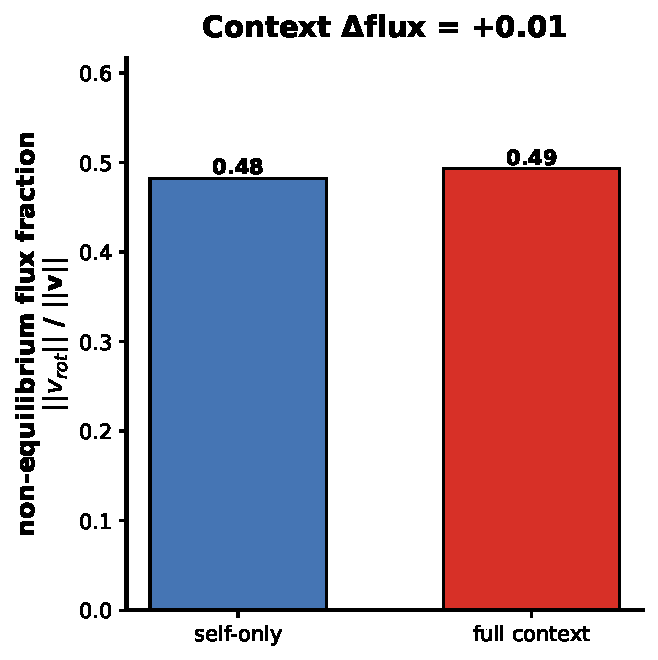
\includegraphics[width=\textwidth]{figures/dynamics/flux_index_self_vs_full_AAH_AIS.pdf}
    \caption{Preinvasive edge (AAH$\rightarrow$AIS).}
    \label{fig:flux-index-self-full-aah}
  \end{subfigure}\hfill
  \begin{subfigure}{0.45\textwidth}
    \centering
    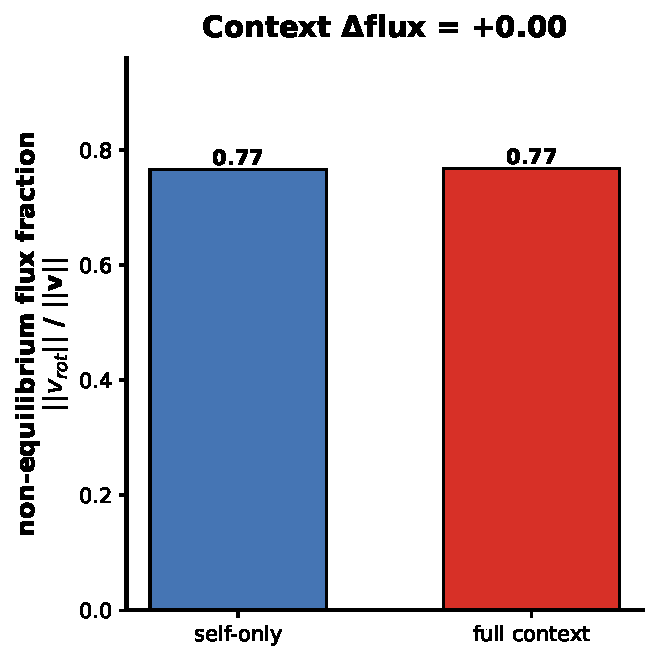
\includegraphics[width=\textwidth]{figures/dynamics/flux_index_self_vs_full_AIS_invasive.pdf}
    \caption{Invasion edge (AIS$\rightarrow$invasive).}
    \label{fig:flux-index-self-full-ais}
  \end{subfigure}
  \caption[Non-equilibrium flux fraction, self-only versus full context]{Scalar non-equilibrium flux
  fraction $\lVert v_{\text{rot}}\rVert/\lVert v\rVert$ (0 = purely gradient/equilibrium, 1 = purely
  rotational) computed for the self-only and full-context fields on each edge. \textbf{(a)} On the
  preinvasive AAH$\rightarrow$AIS edge the fraction is $0.48$ (self-only) versus $0.49$ (full context),
  a context contribution of $+0.01$; \textbf{(b)} on the AIS$\rightarrow$invasive edge it is $0.77$ under
  both fields ($+0.00$). Adding niche context changes the non-equilibrium fraction by at most $+0.01$
  on either edge, so the flux structure is a property of the intrinsic progression field rather than of
  the fitted context perturbation, while the fraction itself is far higher at invasion ($0.77$) than at
  the preinvasive step ($0.48$)---the geometrically more complex reorganization. These are the
  grid-matched headline values quoted in the text and paired with the Helmholtz decomposition of
  Fig.~\ref{fig:helmholtz-decomposition}.}
  \label{fig:flux-index-self-full}
\end{figure}


\begin{figure}[htbp]
  \centering
  \begin{subfigure}{\textwidth}
    \centering
    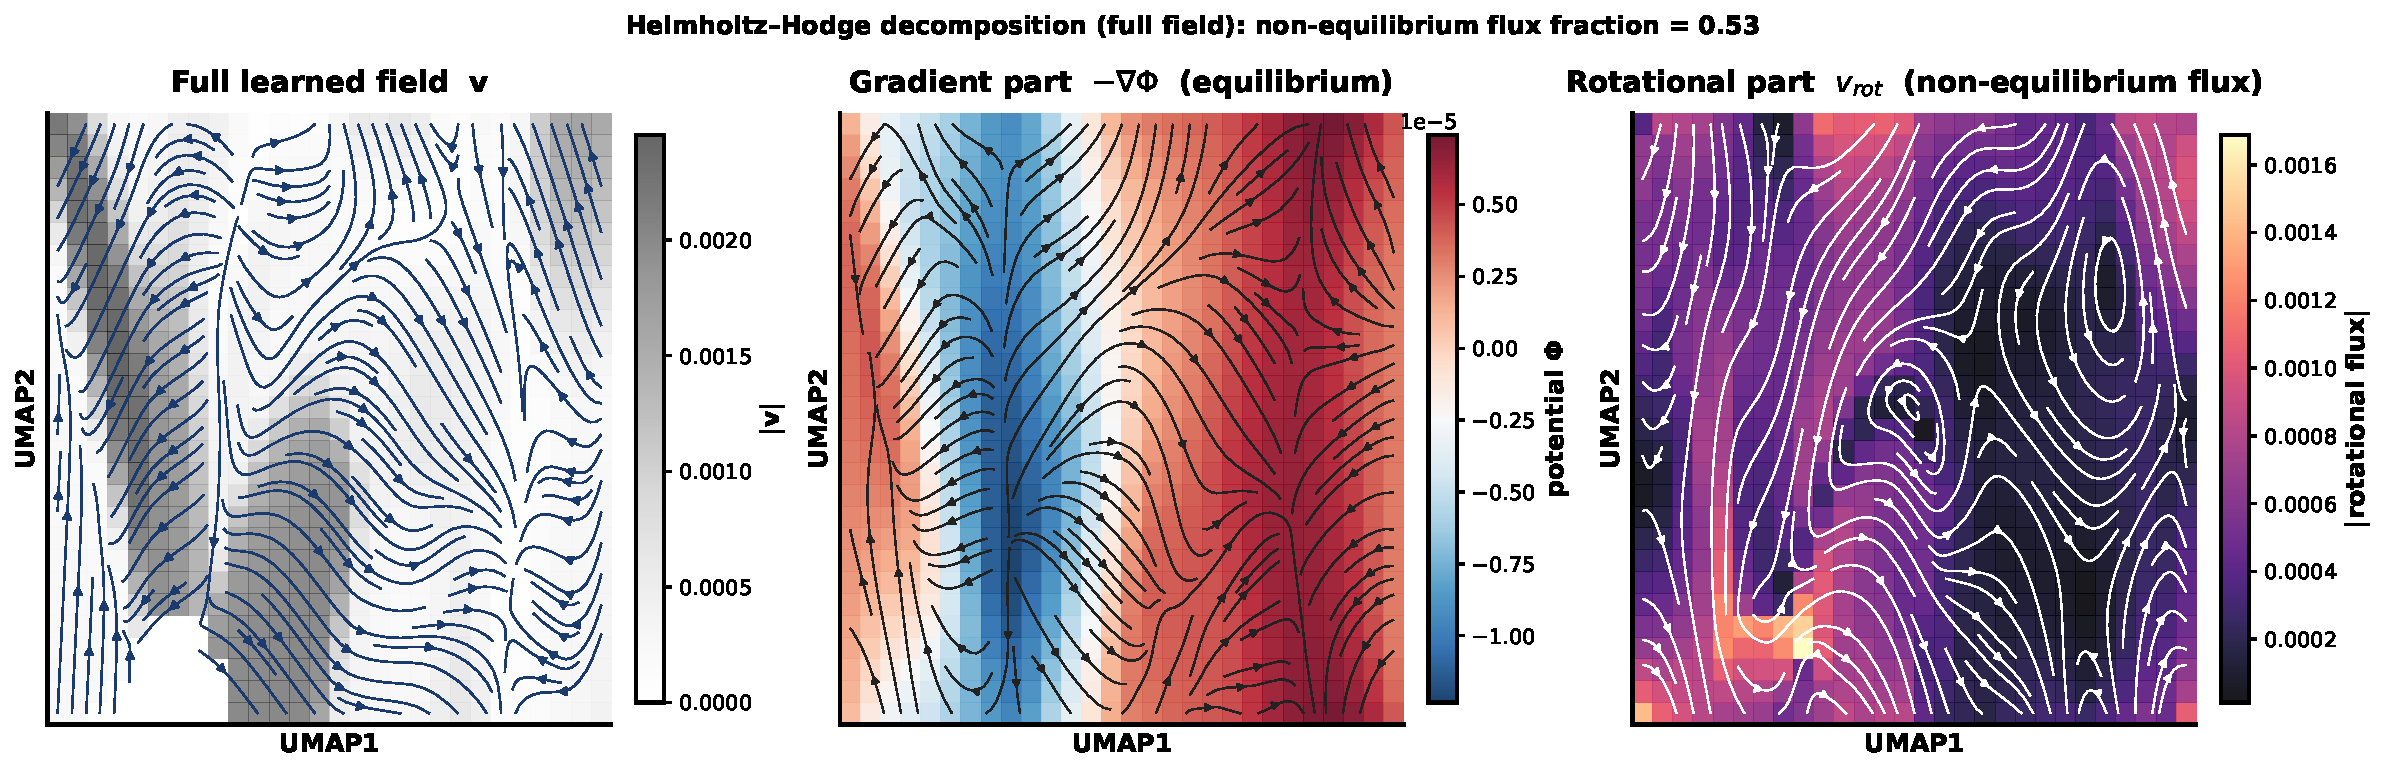
\includegraphics[width=\textwidth]{figures/dynamics/helmholtz_decomposition_full_AAH_AIS.pdf}
    \caption{Preinvasive edge (AAH$\rightarrow$AIS).}
    \label{fig:helmholtz-decomposition-aah}
  \end{subfigure}\\[0.8em]
  \begin{subfigure}{\textwidth}
    \centering
    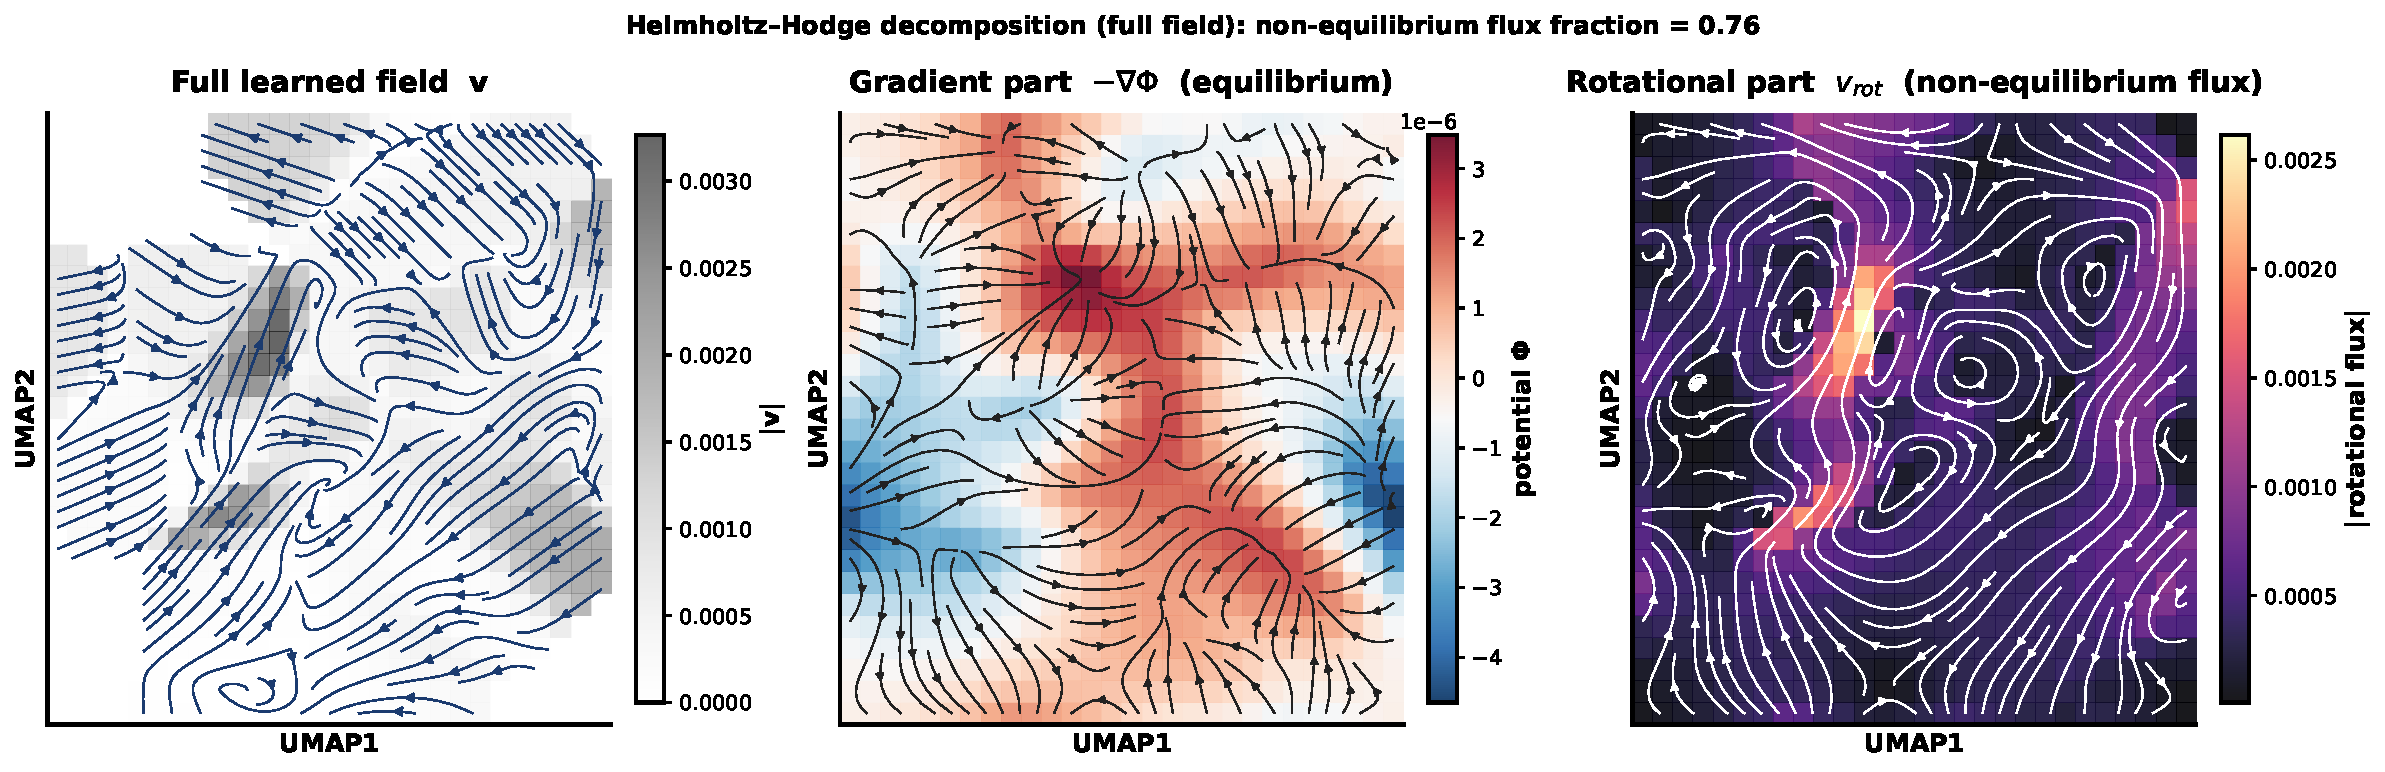
\includegraphics[width=\textwidth]{figures/dynamics/helmholtz_decomposition_full_AIS_invasive.pdf}
    \caption{Invasion edge (AIS$\rightarrow$invasive).}
    \label{fig:helmholtz-decomposition-ais}
  \end{subfigure}
  \caption[Helmholtz--Hodge decomposition of the fitted progression field]{Helmholtz--Hodge
  decomposition of the full (niche-gated) learned field on the receiver UMAP embedding, for each edge.
  Left: the full field $v$ over its speed map. Center: the curl-free gradient part $-\nabla\Phi$ drawn
  over the scalar potential landscape $\Phi$ (the equilibrium, potential-representable component). Right:
  the divergence-free rotational part $v_{\text{rot}}$ (the non-equilibrium circulating flux). Each
  panel's suptitle annotates the non-equilibrium flux fraction $\lVert v_{\text{rot}}\rVert/\lVert
  v\rVert$ evaluated on the $28$-node decomposition grid ($0.53$ on the preinvasive edge, $0.76$ at
  invasion); the grid-matched headline values reported in the text ($0.48$ and $0.77$) are computed on
  the coarser flux-index grid (Fig.~\ref{fig:flux-index-self-full}). \textbf{(a)} The preinvasive edge
  is more nearly gradient-like; \textbf{(b)} the invasion edge carries a larger rotational fraction and
  is therefore less well represented by a pure potential component. The decomposition is applied to a
  deterministic field fitted to pathology-ordered cross-sectional distributions and is descriptive of
  that field's geometry---it is not evidence of a measured thermodynamic flux or a biochemical limit
  cycle.}
  \label{fig:helmholtz-decomposition}
\end{figure}


Hodge decomposition has been applied to RNA-velocity fields to distinguish curl-free, divergence-associated, and cyclic components of cellular dynamics \autocite{Su2024-yq}, and landscape--flux approaches use the coexistence of a potential landscape and non-equilibrium flux to characterize biological systems that cannot be described as simple downhill relaxation \autocite{Wang2008-hd, Wang2011-ai, Zhu2024-it}. In StageBridge, however, the decomposition is applied to a deterministic field learned from pathology-ordered cross-sectional distributions. The rotational component is therefore a property of the fitted vector field, not direct evidence of a biochemical limit cycle, irreversible evolution, or a measured thermodynamic flux. (Fig.~\ref{fig:potential-landscape})

\begin{figure}[htbp]
  \centering
  \begin{subfigure}{0.49\textwidth}
    \centering
    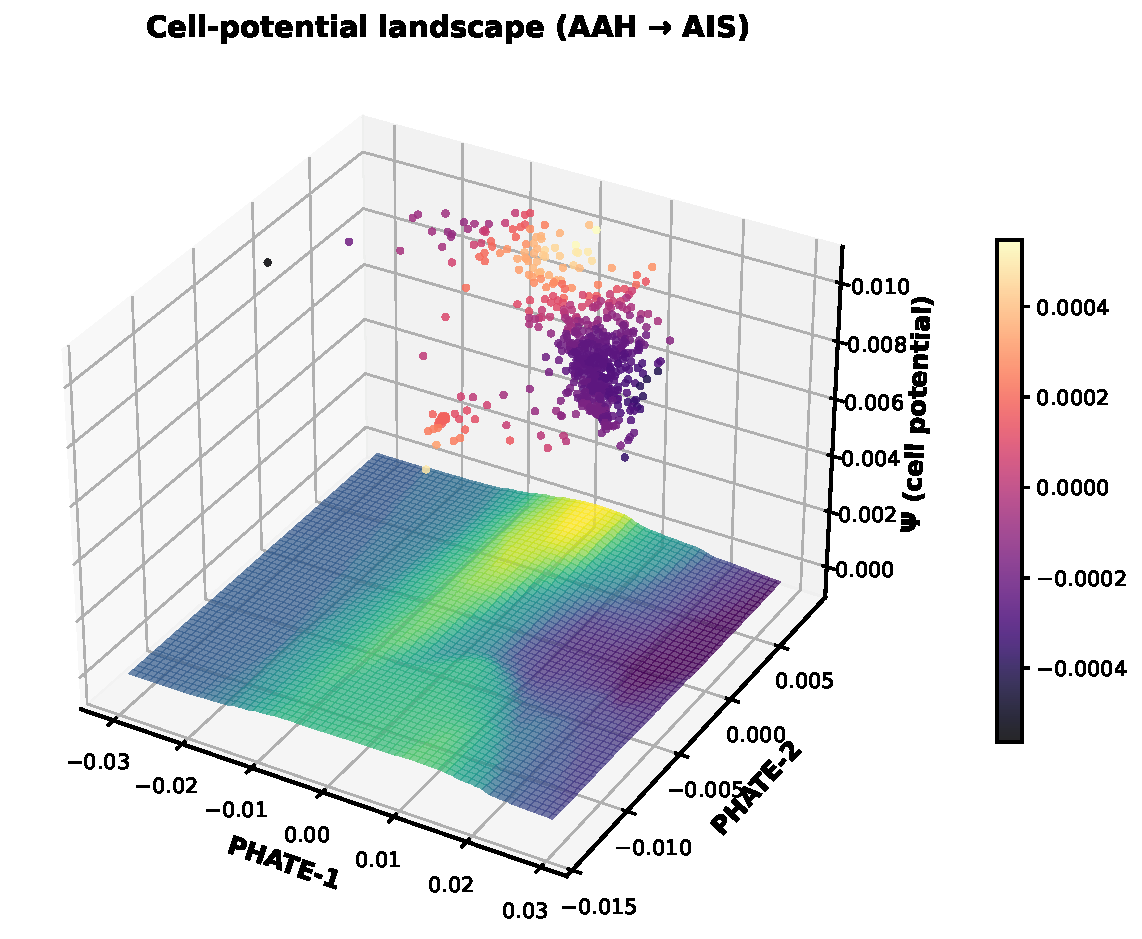
\includegraphics[width=\textwidth]{figures/dynamics/potential_landscape_AAH_AIS.pdf}
    \caption{Preinvasive edge (AAH$\rightarrow$AIS).}
    \label{fig:potential-landscape-aah}
  \end{subfigure}\hfill
  \begin{subfigure}{0.49\textwidth}
    \centering
    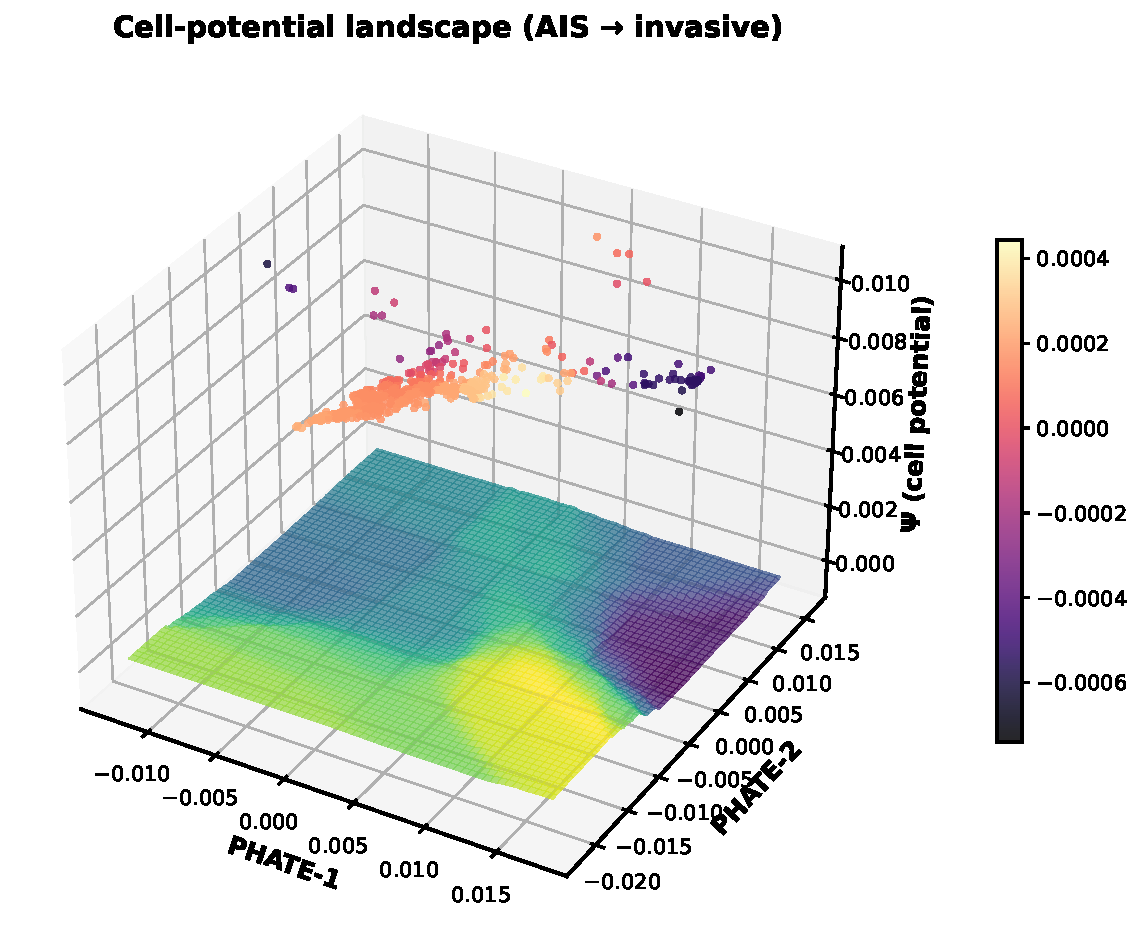
\includegraphics[width=\textwidth]{figures/dynamics/potential_landscape_AIS_invasive.pdf}
    \caption{Invasion edge (AIS$\rightarrow$invasive).}
    \label{fig:potential-landscape-ais}
  \end{subfigure}
  \caption[Fitted potential landscape of the progression field]{The potential-landscape half of the
  landscape--flux description of the fitted field. For each edge the Helmholtz gradient potential
  $\Phi$---the equilibrium component of the decomposition in
  Fig.~\ref{fig:helmholtz-decomposition}---is sampled at every receiver and rendered as a
  Waddington-style surface over the PHATE embedding, with receivers draped on the surface. \textbf{(a)}
  The preinvasive AAH$\rightarrow$AIS edge and \textbf{(b)} the AIS$\rightarrow$invasive edge; the
  invasion field is less fully captured by this gradient/potential component, consistent with its larger
  rotational residual. This surface is the potential of the \emph{fitted transport field} and is
  distinct from the empirical $-\log$ density landscape of Fig.~\ref{fig:waddington}: neither is a
  measured free energy, and the coexistence of this potential with the non-equilibrium flux of
  Fig.~\ref{fig:helmholtz-decomposition} is a geometric property of the learned field rather than a
  thermodynamic claim.}
  \label{fig:potential-landscape}
\end{figure}


The two pathological edges differ in how much of their learned motion can be represented by a gradient component under the same analysis. The result becomes biologically stronger if it is stable across folds, alternative state bases, regularization strengths, and boundary conditions for the decomposition. Those sensitivity analyses should accompany any future claim connecting the rotational component to plasticity, recurrence, or path dependence. Within this thesis, the Helmholtz result supports the conclusion that invasion involves a more geometrically complex reorganization than the earlier transition, while remaining separate from the evidence about the spatial scale of context.

\section{Methodological contribution and relation to prior work}
\label{sec:methodological-contribution}

StageBridge lies at the intersection of population transport, context-conditioned transport, spatial systems biology, and universal differential equations. Waddington-OT established optimal transport as a framework for relating destructive single-cell population snapshots and inferring likely ancestor--descendant correspondences \autocite{Schiebinger2019-lm}. Later work formalized global trajectory recovery across multiple marginals and clarified the assumptions under which trajectories can be inferred from temporal distributions \autocite{Lavenant2023-qv}. These methods provide a transport relation, but they do not define a full-versus-self regulatory contrast for tissue context.

Conditional Monge-map methods such as CondOT learn families of transport maps indexed by experimental or biological context \autocite{Bunne2022-go}. StageBridge shares the goal of context-aware transport but uses context differently: it defines a paired contrast between a full field and a self-only field within a fixed pathological edge, with coarse ecological stratification used to restrict source--target correspondence. Because the implemented transport is an entropy-regularized coupling rather than a uniquely observed lineage, the contribution is more accurately described as a conditional-stratified transport estimand than as recovery of historical cell paths. The broader optimal-transport literature emphasizes this distinction between a model-selected coupling and observed ancestry \autocite{Bunne2024-dv}.

Recent methods also model spatially contextual dynamics more directly. NicheFlow treats whole cellular neighborhoods as evolving point clouds and jointly models cellular states and spatial organization \autocite{Sakalyan2025-ia}. MIOFlow 2.0 incorporates stochasticity, non-conservative growth, and spatial environmental features into a unified trajectory framework \autocite{Sun2026-xk}. OSDR uses single-cell proliferation measurements from one spatial biopsy to identify neighborhood-dependent population dynamics \autocite{Somer2026-ma}. StageBridge is narrower than these models: it holds source context fixed, models epithelial regulatory state rather than population counts or full niche geometry, and asks what modeled endpoint difference is associated with adding context. Its novelty is therefore not the first use of spatial context in a dynamical model, but the combination of a program-resolved context contrast, patient-held-out evaluation, and a falsification ladder designed to distinguish receiver-local information from specimen-level ecology and marginal context structure. The resulting scientific product is also different: StageBridge prioritizes attribution and hypothesis nomination over unrestricted reconstruction of the most flexible possible trajectory.

The universal differential-equation formulation contributes interpretability by separating a structured component from a neural residual, but it also inherits the known challenges of UDEs in sparse and noisy biological systems: optimization instability, overfitting, and competition between the mechanistic and neural components \autocite{Philipps2025-jl}. The unstructured field fit the observed endpoints better than the structured decomposition throughout the falsification ladder. StageBridge therefore makes an explicit trade: lower raw predictive performance in exchange for a program-resolved field and a falsifiable contrast. The relevant unit of interpretation is the composed field and its endpoint contrasts, not individual parameters of the low-rank factorization.

Finally, the transport prior itself is a modeling choice. Entropy-regularized quadratic transport corresponds to a diffusive reference process in a Schrödinger formulation, whereas real gene-expression dynamics can be bursty and non-diffusive. Recent work shows that a mechanistically informed bursty reference process can recover simulated trajectories more accurately than a standard diffusive prior \autocite{Fournie2026-kj}. StageBridge does not resolve that issue, but its frozen benchmark, held-out folds, and negative controls make the consequences of the chosen coupling more visible than they would be in a single unrestricted fit.

\section{Limitations}
\label{sec:discussion-limitations}

Several limitations bound the biological and methodological interpretation.

First, the progression coordinate $\tau$ represents normalized pathological ordering, not elapsed time. StageBridge estimates a field aligned with transitions between stage-labeled distributions; it does not measure transition rates, lesion age, or real-time dynamics. The transport couplings are model-selected correspondences between populations and are not observed lineages. Consequently, the method narrows plausible progression-associated relationships rather than reconstructing the history of an individual cell.

Second, the receiver states are DestVI-decoded epithelial expression profiles derived from mixed-cell Visium spots rather than directly measured single epithelial cells. DestVI provides a principled model for continuous within-cell-type state recovery from spatial mixtures, but its outputs inherit assumptions from the single-cell reference, the generative model, and the assay resolution \autocite{Lopez2022-ps}. Both the epithelial state and its surrounding ecology may therefore contain shared reconstruction error or residual cell-composition signal.

Third, stable-program counts were assessed for patient-held-out and leave-one-donor-out consistency but were not compared with a complete pipeline retrained under permuted context. The current analysis establishes reproducibility under the fitted decomposition; it does not establish enrichment over a retrained context-null model. The endpoint-level local-versus-shuffled comparison is a strong negative control for predictive information, but it is not identical to testing whether the number or identity of stable residual programs exceeds a shuffled-training baseline.

Fourth, donor support was limited. Only two donors contributed epithelial observations to both stages on the principal preinvasive edge, and the AIS$\rightarrow$MIA comparison lacked shared donors. This weakens the ability to distinguish a true within-patient local effect from differences in specimen ecology, pathology, and technical processing. Patient-held-out evaluation prevents direct leakage but cannot create the within-patient counterfactuals absent from the data.

Fifth, context is observed at the source stage and held fixed during integration. The model therefore asks how the same source receiver would move under the fitted full and self-only fields; it cannot represent the niche and receiver co-evolving. This matters because precursor studies increasingly describe reciprocal epithelial, immune, and stromal remodeling \autocite{Peng2025-xu,Takano2024-ys,Cardoso2026-kp,Elhossiny2026-pq}. A source-fixed context effect may combine a true initiating influence with information that, biologically, would change along the trajectory.

Sixth, the structured context field passes through a fourteen-pathway bottleneck before expansion into the full $773$-dimensional regulatory state. Coordination among downstream transcription-factor residuals is therefore partly induced by the architecture. The pathway-level findings sit directly in the gated block and have the strongest attribution. Transcription-factor patterns remain useful for interpretation, but their grouping is less independent than their signs and edge-specific differences. In addition, the neural-residual dominance criterion failed its prespecified interpretability threshold in one of five folds. These features bound confidence in individual regulator-level claims.

Seventh, the regulatory state and transport geometry are Euclidean. Pathway and transcription-factor activity scores are correlated and may occupy a curved or constrained manifold. The transport plan, endpoint distances, fitted field, Helmholtz decomposition, and per-program residual magnitudes all depend on the chosen representation and ground metric. The context-feature variance decomposition is less dependent on this regulatory geometry, but the principal transport quantities are not. Alternative manifold-aware or angular representations are therefore sensitivity analyses rather than automatic improvements.

Eighth, the fitted field is deterministic. A given starting state and context produce one trajectory, while premalignant lesions exhibit heterogeneous outcomes and may progress, remain indolent, or regress. A deterministic field can represent an average tendency but not branch probabilities or stochastic fate selection. The Helmholtz analysis characterizes that deterministic average field; it does not recover hidden branching from cross-sectional data.

Ninth, the context vector is a fixed aggregation of composition and neighborhood summaries rather than a representation learned directly from the constituent cells. The scale of pooling is therefore chosen in advance. Because the central empirical result concerns receiver-local versus specimen-scale information, the encoder's fixed spatial scale is scientifically consequential. A learned encoder might recover a different summary, but increased flexibility would also increase the need for donor support, null retraining, and explicit scale controls.

Finally, the co-expression and communication analyses use the same underlying expression measurements as StageBridge. Their agreement provides internal cross-method consistency, not independent validation. The proposed ligand--receptor--program chains and mechanistic interpretations should therefore be viewed as testable hypotheses for perturbational work.

\section{Future directions}
\label{sec:discussion-future}

The next experiments should follow the inferential hierarchy exposed by the results: first establish whether the program-level residual set exceeds an estimand-level null, then resolve the global-versus-local ecological decomposition, and only afterward increase model capacity or dynamical complexity.

The first priority is a fully retrained shuffle null. The entire context-aware pipeline should be retrained after permuting context within the same stage, donor, and coarse ecological strata, and the number, magnitude, and identity of stable programs should be compared with the observed result. This would determine whether the program-level residual set contains information beyond the inductive bias and capacity of the full model.

The second priority is to make the specimen-versus-local decomposition explicit:

\begin{equation}
  w_i = \bar{w}_{d,s} + \delta w_i,
\end{equation}

where $\bar{w}_{d,s}$ is the donor--stage or specimen-level ecological state and $\delta w_i$ is the receiver-local deviation. The corresponding field should compare

\begin{equation}
\frac{dz_i}{d\tau}
=
 v_{\mathrm{self}}(z_i,\tau)
 + v_{\mathrm{global}}(z_i,\bar w_{d,s},\tau)
 + v_{\mathrm{local}}(z_i,\delta w_i,\tau).
\end{equation}

The decisive test is whether the self+global model is improved by adding local residual context in held-out patients. This formulation targets the unresolved confound directly without requiring a more complicated encoder.

The third priority is to repeat the falsification ladder in data with stronger spatial and patient structure. Takano's use of Visium, Xenium, and multiplexed spatial protein imaging provides one candidate lung resource for cross-resolution testing of epithelial--immune boundaries \autocite{Takano2024-ys}. More generally, cell-resolution assays and cohorts containing multiple stages or lesions from the same patient would determine whether local information was biologically absent, statistically underpowered, or blurred by spot-level measurement.

The discovery workflow should then be tested experimentally. Macrophage- and stromal-derived APOE, GRN, and DCN signaling through LRP1 or EGFR onto FOS- and RB1-associated programs can be evaluated in epithelial organoids, fibroblast or macrophage co-cultures, and targeted ligand or receptor perturbations. The critical design is not simply to ask whether a perturbation changes the endpoint. It is to test whether disrupting a nominated edge selectively reduces the context-associated residual while leaving the self-associated progression component comparatively intact. This directly links the experiment to the StageBridge estimand.

A complementary goal is multimodal validation of how the nominated regulatory programs are molecularly realized. StageBridge currently represents epithelial state using transcript-derived pathway and transcription-factor activities, but transcription does not uniquely determine protein abundance, localization, phosphorylation, acetylation, or signaling activity. Registered spatial transcriptomic and multiplexed protein-imaging data from adjacent sections could test whether StageBridge-nominated programs are accompanied by concordant protein phenotypes at epithelial--immune and epithelial--stromal interfaces \autocite{Takano2024-ys}. Candidate programs showing reproducible RNA--protein discordance could then be evaluated in paired transcriptomic, proteomic, phosphoproteomic, and acetylproteomic lung adenocarcinoma cohorts such as CPTAC LUAD \autocite{Gillette2020-pg}. This analysis should not treat RNA--protein discordance as a direct measurement of post-translational modification. Rather, spatial discordance would nominate regulatory axes for orthogonal testing of translation, protein stability, phosphorylation, acetylation, or compartment-specific signaling. In practical terms, p53 and KAT5/MAML1 nominations could be separated from p53 protein stabilization and acetylation; JAK--STAT residuals could be compared with STAT phosphorylation; WNT residuals could be evaluated against $\beta$-catenin abundance and localization; and epithelial VEGF residuals could be contrasted with endothelial protein-level activity.

A learned neighborhood encoder should be considered only after the explicit global/local contrast is established. A hierarchical Set Transformer can encode unordered sets of neighboring cells and, at a second level, sets of neighborhoods within a specimen \autocite{Lee2019-st}. Its value would be the ability to learn the relevant spatial scale rather than fixing it. Its risk is that it could reconstruct patient or stage identity through high-capacity context features, so it should be evaluated with the same matched shuffles, leave-patient-out folds, and global/local ablations.

The Helmholtz analysis defines a focused computational extension rather than an ornamental visualization. Future work should test whether the increase in rotational fraction at invasion is stable across patient-held-out folds, alternative regularization strengths, different regulatory bases, and alternative decompositions on a graph or manifold. Comparison with Hodge-based analyses of single-cell velocity fields and landscape--flux methods would clarify which aspects are robust geometry and which arise from the learned coordinate system \autocite{Su2024-hd,Zhu2024-lf}. Only after those tests should the rotational component be linked more strongly to path dependence, recurrence, cycling, or non-equilibrium behavior.

Finally, stochastic or branching dynamics would be appropriate in datasets containing information capable of identifying them, such as longitudinal sampling, lineage tracing, calibrated proliferation or loss, repeated lesions, or clinical outcome. Without such anchors, adding stochasticity risks converting uncertainty about the unobserved history into untestable model flexibility. The next version of StageBridge should therefore increase dynamical complexity only when the available measurements can falsify that complexity.

\section{Conclusion}
\label{sec:discussion-conclusion}

This thesis introduced StageBridge to test whether spatial tissue context explains progression-aligned epithelial regulatory change beyond that predicted from the epithelial receiver itself. Across the principal lung adenocarcinoma progression edges, the fitted full-versus-self contrast recovered coordinated program-level residuals that reproduced under patient-held-out and leave-one-donor-out resampling. These residuals nominated biologically coherent changes in checkpoint stress, interferon tone, lineage plasticity, chromatin regulation, and metabolic adaptation, and they provided explicit endpoints for prioritizing sender--ligand--receptor hypotheses. However, receiver-local context did not significantly improve endpoint reconstruction over self-only transport and did not separate from a matched shuffled-context control. The ecological information recoverable from the present cohorts was therefore predominantly specimen-associated rather than uniquely local. The underpowered PanIN analysis returned no stable programs and defined a boundary of available evidence rather than an independent validation. StageBridge should consequently be understood as a falsifiable context-residual estimand with a characterized recovery limit, not as a reconstruction of causal cellular history. Its principal contribution is twofold: it shows how a structured dynamical model can convert otherwise abstract population transport into named, experimentally testable regulatory hypotheses, and it exposes the point at which sparse, cross-sectional spatial observations no longer support the stronger biological claim.
